\documentclass[11pt]{article}
\usepackage[top=1.00in, bottom=1.0in, left=1in, right=1in]{geometry}
\renewcommand{\baselinestretch}{1.1}
\usepackage{graphicx}
\usepackage{natbib}
\usepackage{amsmath}

\begin{document}
\bibliographystyle{/Users/Lizzie/Documents/EndnoteRelated/Bibtex/styles/besjournals}
\renewcommand{\refname}{\CHead{}}

\hspace{-5ex} \includegraphics[width=0.5\textwidth]{/Users/Lizzie/Documents/Professional/images/letterhead/ubc/Faculty of forestry.png}
\pagenumbering{gobble}
\vspace{1.5ex}\\

\setlength{\parindent}{0pt}
\setlength{\parskip}{7pt}
\today

Dear Dr. Gelman, MacElreath and Vehtari:

We would be grateful for your consideration of whether our manuscript, ``A four-step simulation-based workflow for improving ecological science,'' may fit as an Opinion (or other article type) in your special issue in \emph{Philosophical Transactions A}.

Ecology is a discipline facing increasing challenges given growing demands and historical statistical practices. Ecologists are now often asked for models that can provide useful forecasts and predictions, driving them towards more complex models to leverage larger datasets \citep{anderson2021trends,muff2022rewriting}. But many researchers---ourselves included---were not trained in the best statistical practices for these approaches, and thus often rely on a limited set of pre-defined models combined with null hypothesis testing \citep{quinn1983hypothesis,hobbs2006alternatives}. The result is poor models that lead to incorrect predictions and decisions, alongside concerns of a looming replication crisis \citep{filazzola2021replication,fraser2020role} in a field that has become increasingly policy-relevant \citep{hak2016sustainable,lindenmayer2010science}.  While many ecologists may not be formally trained in the fitting of large, complex models, a large number have the computational toolkit to approach such models, but lack an organizational framework to develop, test and improve bespoke models. 

To address this gap, we outline a generalizable workflow built from those developed in statistics  \citep{gelman2020bayesian,grinsztajn2021,vandeschoot2021} that introduces ecologists to more robust model construction through a focus on simulations. Building on new insights from statistics and data science \citep{gelman2020bayesian}, this approach moves away from a focus on null hypothesis testing, traditionally a mainstay of ecology, towards estimating effect sizes, using models calibrated and better understood through simulating data at multiple steps---using a number of skills more often associated with theoretical than empirical ecology. We then outline one such iterative workflow, which contains four steps (see Fig. \ref{fig:workflow} below) that will be approachable to ecologists,  highlighting how it has changed our science and how it may improve statistical and mathematical training in ecology. We argue this example for the field of ecology could provide a blueprint for other fields that have not yet taken up workflow-approaches formally. 

The workflow follows the basics of how authors EM Wolkovich, TJ Davies and WD Pearse approach model building and leverages the insights and skills of computational statistician M Betancourt. We have designed it to be broadly generalizable and practical, including relevant examples of estimating shifts in animal and plant timing over recent decades. % To make sure the steps are clear and accessible we would present full example of the workflow and accompanying code (in R Markdown) to estimate trends over time in plant and animal phenology. 

We hope that you will find this perspective, which provides a road-map for the many ecologists now building more complex models, suitable for publication in your special issue. By integrating simulation more fully in model building and testing this workflow can fit models that are more robust and well-suited to provide new ecological insights---allowing us to refine where to put resources for better estimates, better models, and better forecasts. % 

Sincerely,\\

\includegraphics[scale=1]{/Users/Lizzie/Documents/Professional/Vitas/Signatures/SignatureLizzieSm.png} \\

Elizabeth M Wolkovich\\
Associate Professor of Forest \& Conservation Sciences\\ 
University of British Columbia\\

{\bf References}
\vspace{-8ex}
\bibliography{..//refs/bayesrefsmini.bib}


\vspace{5ex}

\begin{figure}[ht]
\centering
\noindent 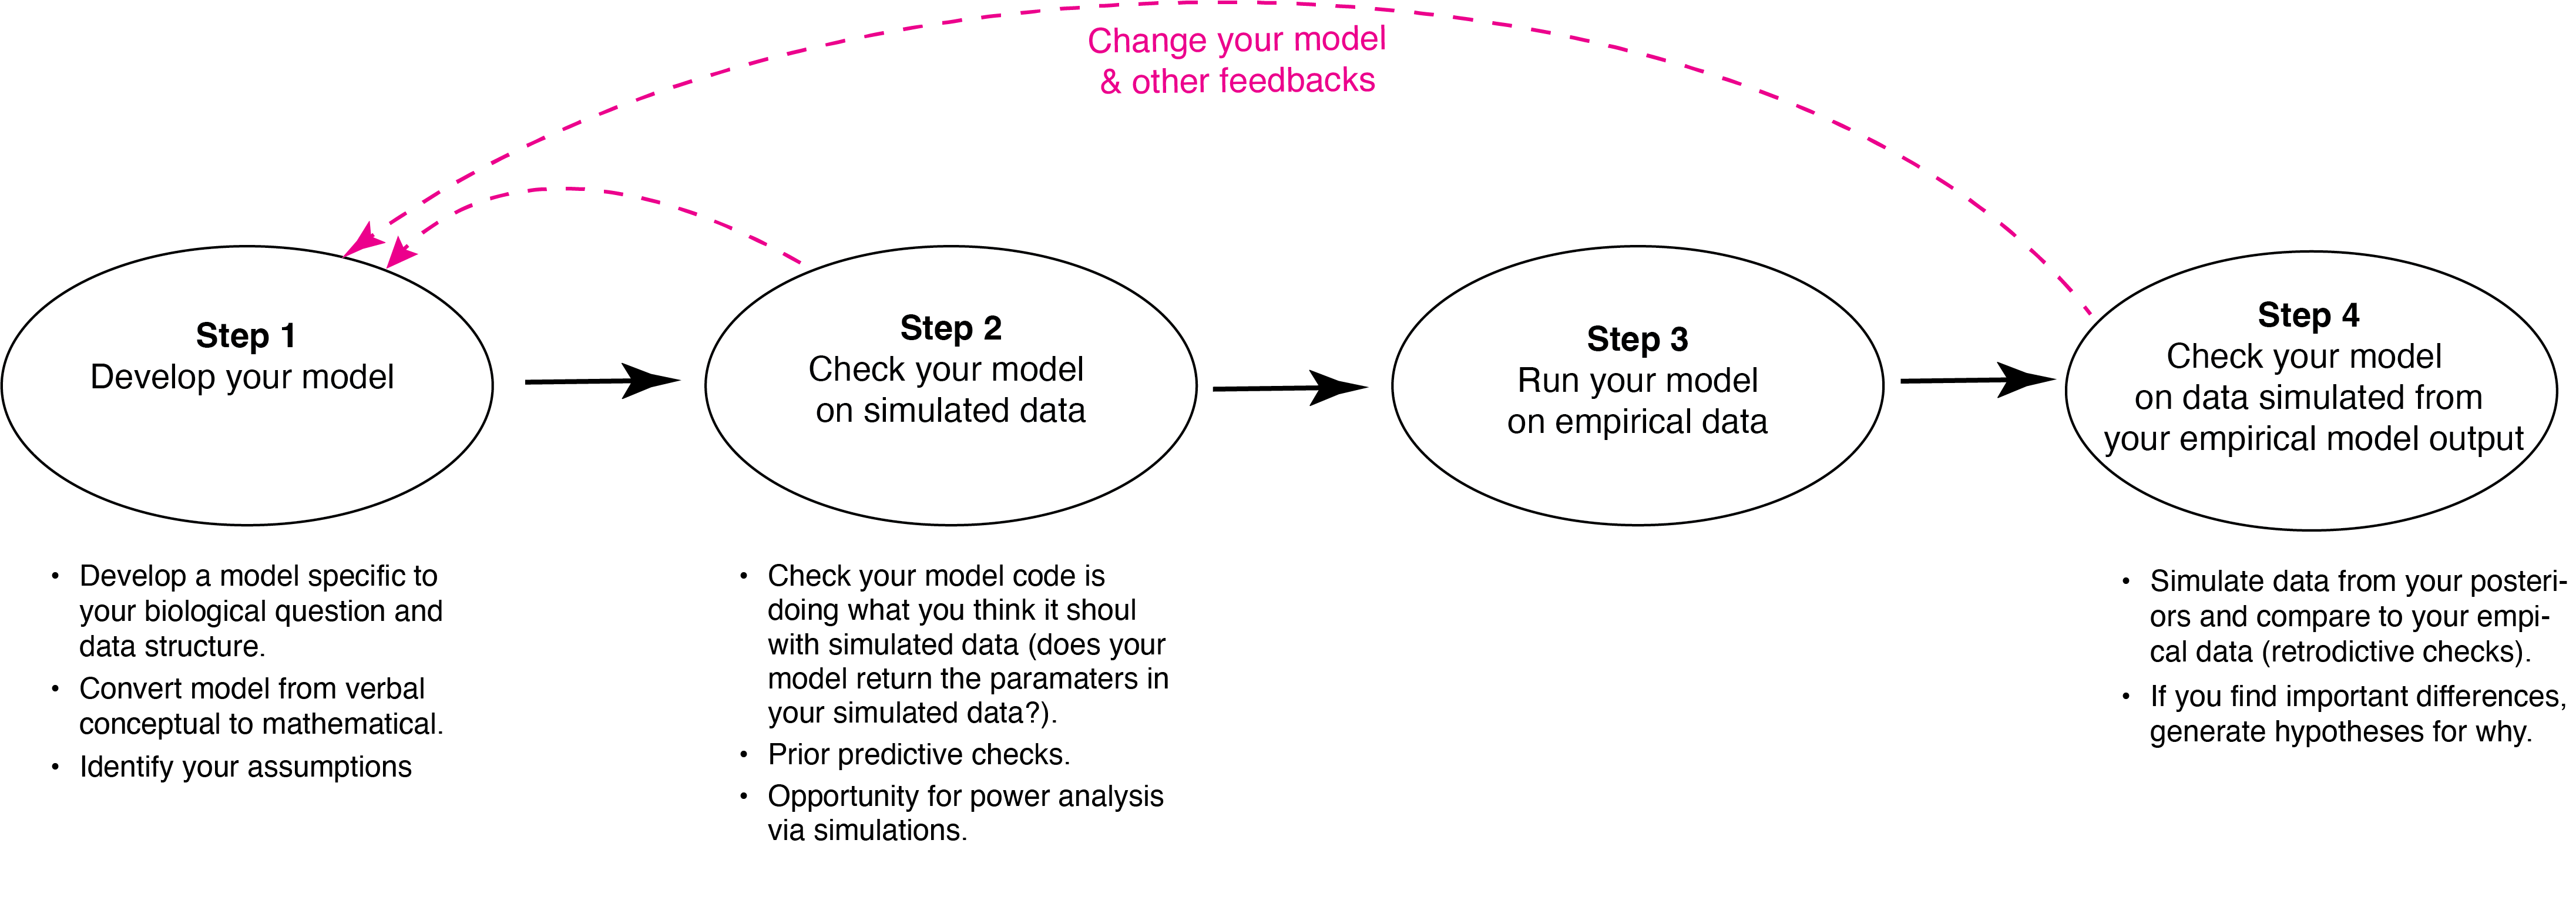
\includegraphics[width=1\textwidth]{..//figures/workflow.png}
\caption{The four-step iterative workflow we outline can help design models for specific ecological questions, data and aims---which makes this a statistical workflow that can naturally become a scientific workflow. It makes the step that many ecologists focus on---running your model on your empirical data (Step 3)---far more straightforward and insightful by using simulations both before (Step 2) and after (Step 4) it to better understand the model and data together.}
\label{fig:workflow}
\end{figure}


\end{document}

\newpage
{\bf Example figures}





%%%
%%%


\begin{figure}[ht]
\centering
\noindent 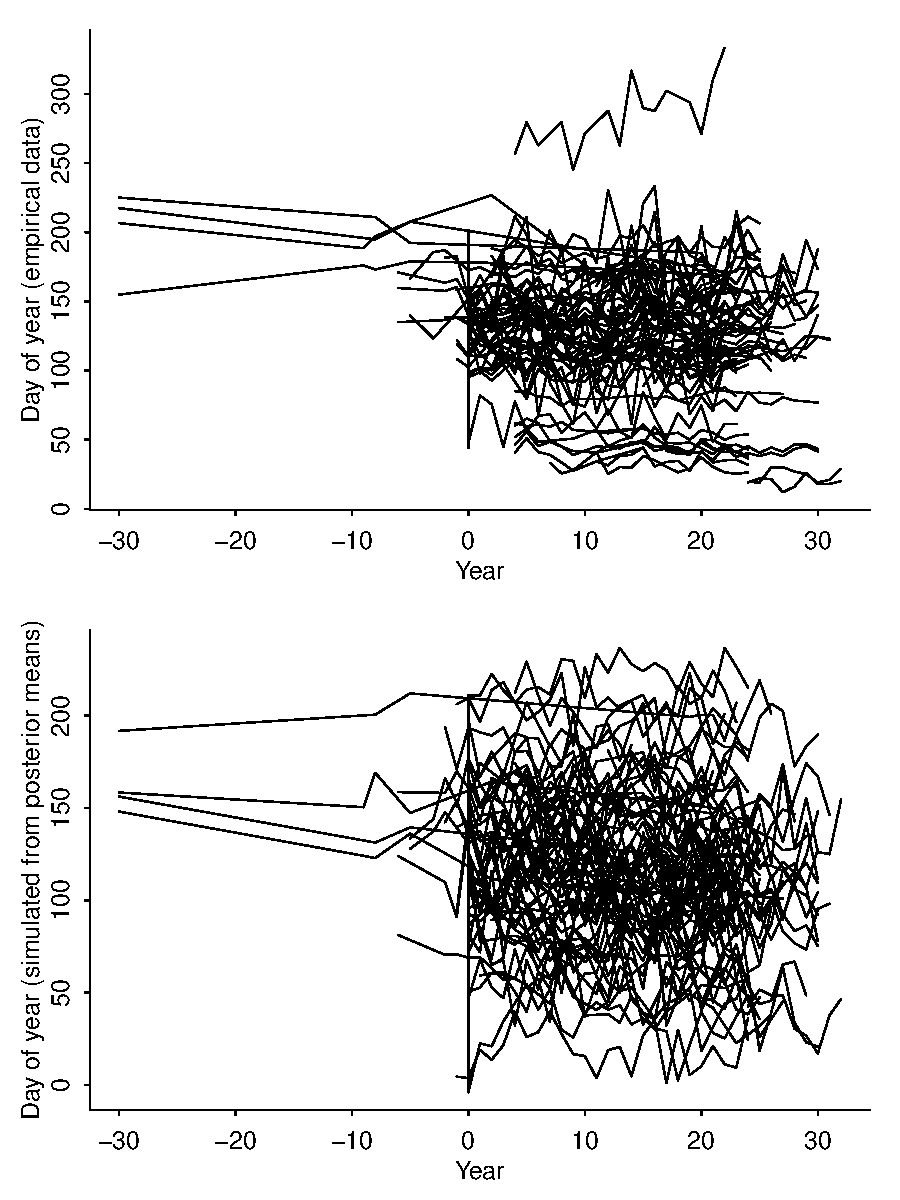
\includegraphics[width=0.6\textwidth]{..//examples/synchrony/graphs/rawvsonepredictivecheck.pdf}
\caption{Example of a single retrodictive check from time-series data of phenological events over time. The raw data (top, black) looks similar to one simulated dataset (bottom, purple), based on existing species number, their respective $x$ data, and simulating from the parameters for each species. See `An example workflow' in the Supplement for more details.}
\label{fig:retrodictivecheck}
\end{figure}

\begin{figure}[ht]
\centering
\noindent 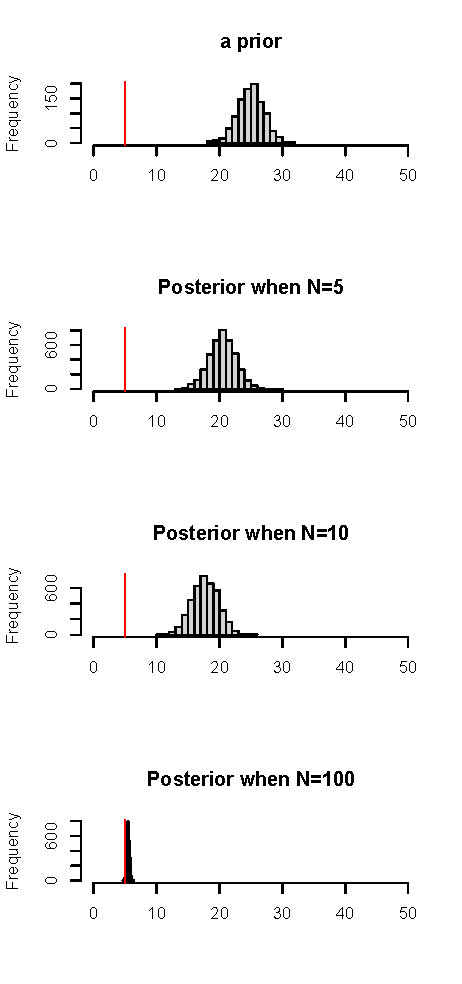
\includegraphics[width=0.5\textwidth]{..//examples/misspecifiedmodel/priorpostforflows.pdf}
\caption{A simple example of how to use simulated data to understand calibration issues in a mis-specified model. Here we know the true model underlying the data is $y=\alpha + \text{normal}(0, \sigma)$ where $\alpha$ is 5 (shown as blue vertical line) and $\sigma$ is 2. The model, however, is mis-specified by a prior for $\alpha$ of $\text{normal}(25, 2)$ (dashed blue line), resulting in a posterior (salmon-colored histogram) not centered on the true value. In our experience it is quite rare to have a prior informed by ecological knowledge be so far off, but this is an example. How mis-calibrated the model will be depends on the data: we show examples with a sample size ($N$) of 5, 10 and 40 data points. In practice these studies would allow us to determine how much data we would need to be robust to suspect prior models. (Note the change in $y$ axis range for bottom plot.) }
\label{fig:misspecifyprior}
\end{figure}


